\documentclass{article}
\usepackage[utf8]{inputenc}
\usepackage{amsmath,amsfonts,amssymb} % Paquetes para matemáticas
\usepackage{ulem} % Para subrayar texto
\usepackage{geometry}
\usepackage{indentfirst}
\usepackage{graphicx}
\usepackage{float}
\usepackage[backend=biber,style=apa]{biblatex}
\addbibresource{bibliografia.bib}

\geometry{
    a4paper,
    left=2cm,
    right=2cm,
    top=2.5cm,
    bottom=2.5cm,
    includefoot,
    headheight=15pt,
    headsep=0.5cm,
    footskip=1cm
}

\title{TP2 - Gestión eficiente de recursos en sistemas ferroviarios}
\author{Candelaria Sutton, Dafydd Jenkins, Josefina Jahde}
\date{\today}

\begin{document}

\maketitle

\section*{Introducción}
En este trabajo, abordamos el problema de la planificación y gestión óptima del material rodante para una empresa ferroviaria. El problema consiste en definir una asignación eficiente de material rodante a las distintas estaciones cabecera de una linea ferroviaria. Se busca minimizar el número total de unidades de material rodante necesarias para cubrir la demanda de la línea en cada horario, considerando que es posible la reutilzación de unidades entre viajes.

Este problema pertenece a la categoría de problemas de circulación en redes y tiene gran relevancia en la optimización de recursos en operaciones logísticas y de transporte. En el contexto de la industria ferroviaria, una asignación ineficiente del material rodante (trenes) puede llevar a costos innecesarios y al uso ineficiente de los recursos disponibles, afectando tanto a la empresa como a los usuarios del servicio.

El objetivo de este trabajo es desarrollar un modelo que permita resolver el problema de circulación de trenes utilizando algoritmos de flujo de costo mínimo. Además, se implementará un set de experimentos para analizar el rendimiento del modelo en diferentes escenarios de demanda y costos.

En este informe se pueden encontrar las secciones:
\begin{itemize}
    \item Sección 1: se describe el problema, las restricciones y las consideraciones del mismo.
    \item Sección 2: se describe la metodología, explicando cómo se modeló el problema y se implementó dicho modelo.
    \item Sección 3: detalla los experimentos realizados, presentando hipótesis, diseño de pruebas y resultados obtenidos.
    \item Sección 4: se analiza el $Escenario Adicional$ propuesto por la cátedra.
    \item Sección 5: se presentan las conclusiones, discutiendo la efectividad del modelo y posibles extensiones para trabajos futuros.
\end{itemize}

\section*{Sección 1: El problema}
El problema consiste en definir una asignación eficiente de material rodante a las distintas estaciones cabecera de una linea ferroviaria. Se busca minimizar el número total de unidades de material rodante necesarias para cubrir la demanda de la línea en cada horario, considerando que es posible la reutilzación de unidades entre viajes. Para cada viaje que se realiza en la línea durante un día, se tiene la demanda en cantidad de pasajeros y las estaciones y horarios de salida y llegada. Además se cuenta con restrcciones: cantidad máxima de unidades que pueden circular por la línea y la capacidad máxima (en pasajeros) de cada unidad.

Se toma una versión simplificada con las siguientes consideraciones:
\begin{itemize}
    \item Los traspasos de unidades ocurren únicamente en las cabeceras de la línea.
    \item Se pueden almacenar infinita cantidad de unidades de material rodante en las cabeceras.
    \item Todos los servicios tienen el mismo tipo de unidad rodante (en cuanto a cantidad de pasajeros).

\end{itemize}

\section*{Sección 2: Modelado e implementación}
Para la resolución del problema, se adaptó  el modelo propuesto por \textcite{schrijver}. Dicho modelo se realiza a partir del cronograma, la informacion sobre la demanda y las restricciones de los servicios que recorren una linea durante el día, usando un digrafo que modele una red espacio-tiempo. Se formula la decisión como un problema de Circulación sobre la red que se reduce a un problema de Flujo de Costo Mínimo y se resuleve utilizando algoritmos de flujo. Tanto para la construcción de la red como para los algoritmos de flujo se utilizó la librería $NetworkX$ de Python.

\subsection*{Creación del Grafo}

La resolución comienza con la construcción del digrafo de la red. El mismo contiene un conjunto de vértices $V$, donde cada vértice representa un evento de llegada o salida a una estación. Dicho nodo tiene como etiqueta el nombre de la estación y el horario correspondiente y posee un imbalance igual a 0. Además, se agregan dos nodos que representan el final del día de cada estación, con etiqueta  \texttt{\{estacion\}\_0} (porque es un evento que ocurre a las 00:00).

El conjunto $A$ de arcos del digrafo está compuesto por tres tipos:

\begin{itemize}
    \item de tren: $(i, j)$ conecta el evento de partida y el de arribo de un servicio, representando el viaje del servicio desde su estacion origen a su estación destino. Estos arcos cuentan con una cota inferior $l_{ij}$ de la cantidad de unidades necesarias para satisfacer la demanda y una cota superior $u_{ij}$ de la cantidad maxima de unidades que pueden circular en un servicio. El costo es $c_{ij} = 0$.
    \item de traspaso: $(i, j)$ conecta dos eventos consecutivos (en tiempo) dentro de una estación, indicando el pasaje de unidades entre eventos. Esta arista tiene cota inferior $l_{ij} = 0$, $u_{ij} = \infty$ y costo $c_{ij} = 0$.
    \item de reordenamiento: $(i, j)$ conecta los eventos del final del dia de cada estación mutuamente. Simula el pasaje de unidades entre estaciones una vez que terminó el día. Estas aristas tienen cota inferior $l_{ij} = 0$, $u_{ij} = \infty$ (si bien son unidades viajando por la línea, se asume que se podrían hacer tantos viajes como fuesen necesarios), y costo $c_{ij} = 0$ (no implican agregar unidades extra a la línea).
    \item de trasnoche: una para cada estación, conectan el ultimo evento del día (el nodo de final del día) con el primero. Modela las condiciones de borde respecto que la cantidad de unidades al finalizar el día en una estación debe ser la necesaria para poder iniciar las operaciones al día siguiente. Estos arcos tienen $l_{ij}= 0$, $u_{ij} = \infty$ y $c_{ij} = 1$. Además, estos arcos son los utilizados para obtener la cantidad de unidades de material rodantes necesarias en la línea.
\end{itemize}

Tomando como ejemplo la \texttt{toy\_instance} provista por la cátedra, el grafo quedaría como se muestra a continuación:

\begin{figure}[H]
    \centering
    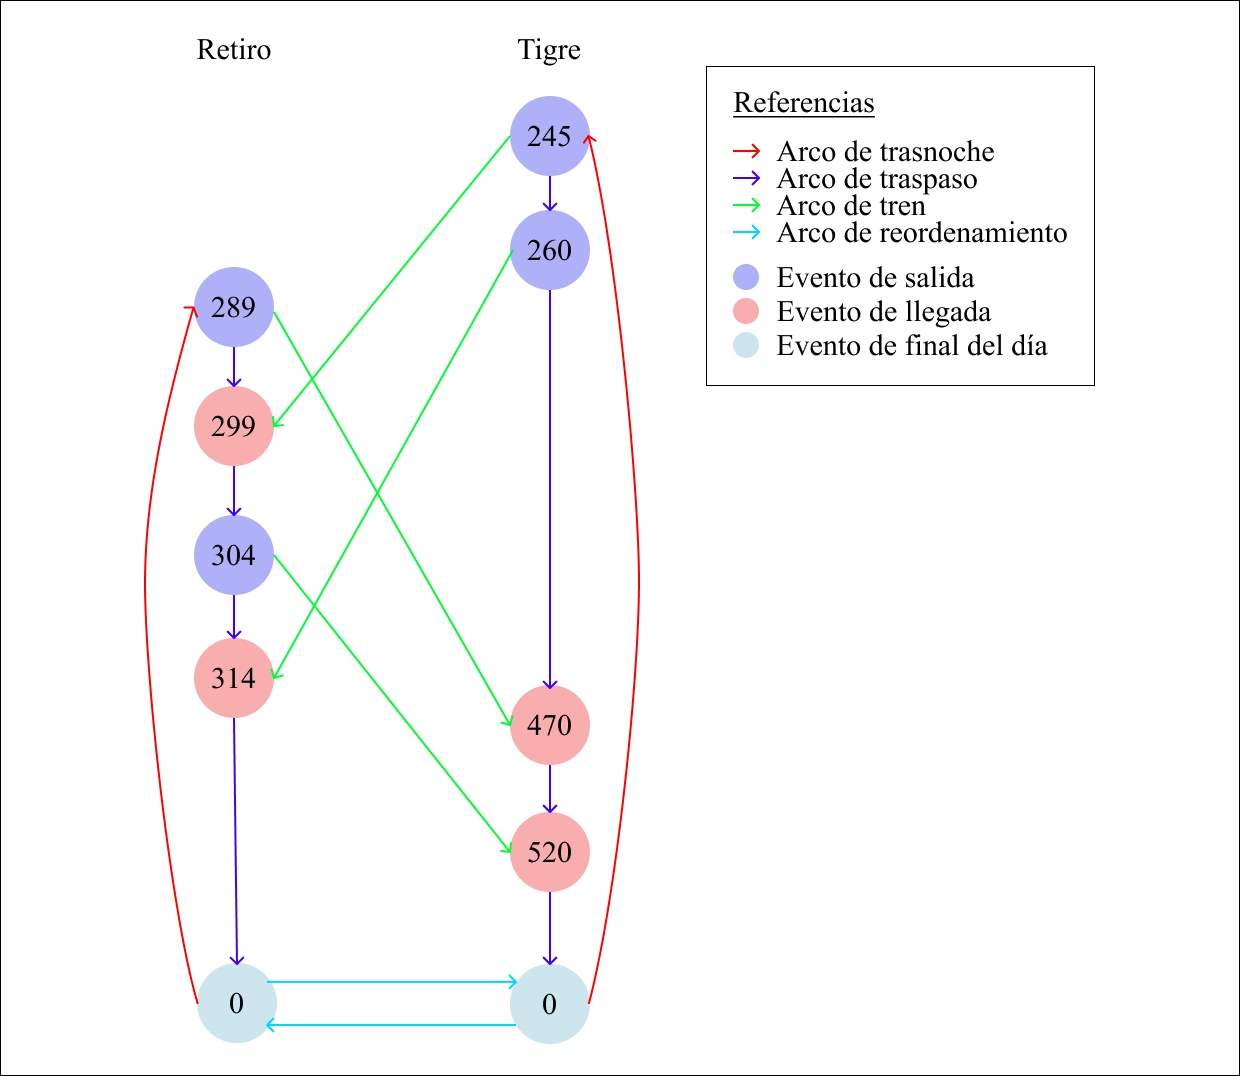
\includegraphics[width=0.60\textwidth]{esquema_toy_instance.png}
    \caption{Grafo para \texttt{toy\_instance}}
    \label{fig:ejemplo}
\end{figure}

La construcción del grafo se realiza con el método \texttt{create\_graph()} que, al igual que todos los demás métodos de esta implementación, se encuentra implementado en el archivo \texttt{railway\_service.py}. 

\subsubsection*{Entrada del Algoritmo}

El algoritmo recibe un diccionario \texttt{data} con la siguiente estructura:

\begin{itemize}
    \item \texttt{data["services"]}: Diccionario que contiene los servicios, incluyendo horarios de salida y llegada, y demanda de pasajeros.
    \item \texttt{data["rs\_info"]["capacity"]}: Capacidad del material rodante (RS).
    \item \texttt{data["rs\_info"]["max\_rs"]}: Número máximo de unidades de RS disponibles.
    \item \texttt{data["stations"]}: Lista de estaciones, cabecera.
\end{itemize}

\subsubsection*{Proceso del Algoritmo}

\begin{enumerate}
    \item \textbf{Inicialización}: 
    Se crea un grafo dirigido \texttt{G} utilizando NetworkX y se define un diccionario \texttt{nodos\_estacion} para almacenar los tiempos de salida y llegada de cada estación.

    \item \textbf{Creación de Nodos y Aristas de Servicios}:
    Para cada servicio en \texttt{data["services"]}, se extraen los horarios de salida y llegada, y se crean etiquetas para los nodos (\texttt{salida\_str} y \texttt{llegada\_str}). Se calcula la cantidad de RS necesarios y se crean aristas con:
    \begin{itemize}
        \item \textbf{Peso (\texttt{weight})}: 0, ya que no hay costo asociado al servicio.
        \item \textbf{Cota mínima (\texttt{lower\_bound})}: Igual al número de RS necesarios para cumplir la demanda.
        \item \textbf{Cota máxima (\texttt{upper\_bound})}: Igual al máximo número de RS disponibles.
    \end{itemize}

    \item \textbf{Creación de Nodos de Final del Día}:
    Se agregan nodos adicionales para representar el final del día en cada estación (\texttt{final\_a} y \texttt{final\_b}), y se conectan entre sí con aristas para permitir el traspaso de material rodante.

    \item \textbf{Creación de Aristas Internas en las Estaciones}:
    Para cada estación, se ordenan los tiempos de salida y llegada, y se crean aristas dirigidas entre tiempos consecutivos dentro de la misma estación, con:
    \begin{itemize}
        \item \textbf{Peso (\texttt{weight})}: 0.
        \item \textbf{Cota mínima (\texttt{lower\_bound})}: 0.
        \item \textbf{Cota máxima (\texttt{upper\_bound})}: 1e9.
    \end{itemize}

    \item \textbf{Creación de Aristas Cíclicas en las Estaciones}:
    Se conectan el último nodo de cada estación con el primer nodo de la misma estación, con un costo (\texttt{weight}) de 1.

\end{enumerate}

\subsubsection*{Salida del Algoritmo}

El método devuelve:
\begin{itemize}
    \item \texttt{G}: El grafo dirigido que modela el problema de circulación, con nodos etiquetados con horarios y aristas con atributos de imbalance, capacidad máxima y cota mínima.
    \item \texttt{nodos\_estacion}: Un diccionario con los tiempos de salida y llegada de cada estación, ordenados de menor a mayor.
\end{itemize}

\subsection*{Resolución del problema de Circulación mediante reducción al problema de Flujo de Costo Mínimo}
Para la reducción del problema de Circulación a un problema de Flujo de Costo Mínimo, se toma el grafo construído y se construye uno nuevo con las siguientes modificaciones:
\begin{itemize}
    \item Para cada nodo $i$ el imbalance $b_i$ es:
$$
\begin{aligned}
b_i = \sum_{j \in N^-(i)} l_{ji} - \sum_{j \in N^+(i)} l_{ij}
\end{aligned}
$$
    \item Para cada arco, su nueva capacidad $\hat{u}_{ij}$ será $\hat{u}_{ij} = u_{ij} - l_{ij}$
\end{itemize}

Sea $\hat{x}^*$ la solución del problema de flujo de costo mínimo definido anteriormente,  $x^*_{ij} = l_{ij} + \hat{x}^*_{ij}$ es una solución óptima del problema de circulación original.

La transformación anteriormente descrita se implementa en el método \texttt{solve\_circulacion()}. 

\subsubsection*{Entrada del Algoritmo}
El algoritmo recibe como parámetro el grafo \texttt{G} del problema de Circulación.

\subsubsection*{Proceso del Algoritmo}

\begin{enumerate}
    \item \textbf{Inicialización}: 
    Se crea un digrago \texttt{H} utilizando el método \texttt{transform\_graph()} que realiza la transformación del grafo según se describió anteriormente. Este método define \texttt{H} como digrafo, le agrega los nodos de \texttt{G} y las aristas del mismo pero con la capacidad correspondiente según la transformación. Luego modifica los imbalances de los nodos según la transformación, recorriendo todo arco y sumándole al nodo de salida el $l_{ij}$ y restándoselo al nodo de entrada. 

    \item \textbf{Resolución del problema de Flujo de Costo Mínimo}:
    Para el grafo \texttt{H} se resuelve el problema de Flujo de Costo Mínimo usando el método \texttt{min\_cost\_flow()} de \texttt{NetworkX}. Este método devuelve un diccionario que contiene para cada arco saliente de cada nodo de \texttt{H} el flujo que circula por dicho arco. Dicho diccionario se almacena en \texttt{circulacion}

    \item \textbf{Transformación del Flujo de Costo Mínimo a la Circulación}:
    Se recorren los nodos \texttt{u} del flujo de los que salen arcos. Para cada uno de sus vecinos \texttt{v}, se modifica \texttt{circulacion} sumándole a la arista \texttt{u$\rightarrow$v} el $l_{ij}$.

\end{enumerate}

\subsubsection*{Salida del Algoritmo}
Se retorna el diccionario \texttt{circulacion} que contiene, para cada arco saliente de cada nodo, el flujo que circula por dicho arco.

\subsection*{Generación de la respuesta final (cantidad de unidades necesarias)}
Para calcular la cantidad total de unidades necesarias, se suma el flujo circulante por las aristas de trasncohe. Para ello se utiliza el método implementado \texttt{get\_cost()}.

\subsubsection*{Entrada del Algoritmo}
El algoritmo recibe como parámetros

\begin{itemize}
    \item el grafo \texttt{G} del problema de Circulación.
    \item el diccionario \texttt{circulación} resultante de \texttt{solve\_circulacion()}.
    \item el diccionario \texttt{nodos\_estacion} resultante de \texttt{create\_graph()} (para obtener las etiquetas del primer y último nodo de cada estación).
\end{itemize}

\subsubsection*{Proceso del Algoritmo}

\begin{enumerate}
    \item \textbf{Cálculo del costo resultante}:
    Se inicializa el costo resultante \texttt{cost} incialmente igual a 0.
    Sean las estaciones $x, y$ se recorren las posibles combinaciones $(a, b)$ para $a, b \in \{x, y\}$. Para cada combinación se define \texttt{begin} como el primer nodo de $a$, y  \texttt{end} como el último nodo de $b$. Finalmente, se suma a \texttt{cost} el flujo circulante por el arco $\texttt{end}\rightarrow\texttt{begin}$.

\end{enumerate}

\subsubsection*{Salida del Algoritmo}
Se retorna \texttt{cost}, el costo resultante de sumar el flujo circulante por las aristas de trasnoche.

\subsection*{Otros métodos}
Se implementaron otros métodos para facilitar la implementación de los algoritmos, la experimentación y el uso por parte de los usuarios. A continuación se describe la funcionalidad que cumple cada uno y el modo de uso esperado para aquellos usuarios que desearan realizar sus propias experimentaciones.

\begin{itemize}
	\item \texttt{load\_instance()}: recibe la ruta un archivo json, a partir del cual generar una instancia de cronograma para resolver el problema.
	\item \texttt{show\_graph()}: recibe un grafo \texttt{G} y el diccionario \texttt{nodos\_estacion} generados por el método \texttt{create\_graph()} y una instancia de cronograma \texttt{data}. Muestra el grafo ubicando los nodos de cada estación por columnas. Muestra en los arcos la cota mínima $l$ y capacidad $u$.
	\item \texttt{show\_flow()}:   recibe un grafo \texttt{G} y el diccionario \texttt{nodos\_estacion} generados por el método \texttt{create\_graph()}, una instancia de cronograma \texttt{data} y el flujo \texttt{flow} resultante del método \texttt{solve\_circulacion()}. Muestra el flujo en el grafo \texttt{G}.
	\item \texttt{modelo\_circulacion()}: recibe una instancia de cronograma \texttt{data}. Resuelve el problema de circulación para la instancia haciendo uso de los métodos \texttt{create\_graph()}, \texttt{solve\_circulacion()} y \texttt{get\_cost()}, y devuelve el la cantidad de unidades necesarias para resolver el problema.
	\item \texttt{modelo\_empresa()}: recibe una instancia de cronograma \texttt{data}. Resuelve el problema utilizando el método de la empresa y devuelve la cantidad de unidades necesarias. Para ello,

\begin{enumerate}
    \item Se inicializan contadores para el stock  y la cantidad de unidades nuevas de cada estación en 0.

    \item Se almacenan los eventos de  \texttt{data} como tuplas y se las ordena según el horario.

    \item Para cada evento, si es una llegada, se suman las unidades recibidas (iguales a lo minimo necesario para cubrir la demanda) al stock de la estación. Si es una salida, se trata de cubrir la demanda con el stock disponible. Si este es insuficiente, el remanente se obtiene incrementando la cantidad de unidades nuevas.

    \item Se devuelve la cantidad de unidades nuevas para cada estación.
\end{enumerate}

\end{itemize}

Para mayor claridad, en los archivos \texttt{uso\_funciones.py} y \texttt{main.py} de la carpeta \texttt{src} se pueden ver ejemplos de uso de los métodos implementados.

Finalmente, los algoritmos desarrollados e implementados se testearon con la instancia \texttt{toy\_instance} propuesta por la cátedra y otras instancias que representan distintos casos bordes. Dichas instancias se encuentran en la carpeta \texttt{test} y son:

\begin{itemize}
	\item \texttt{catch\_and\_shoot}: caso en el que cada salida de una estación se puede cubrir con stock existente en la misma proveniente de una llegada previa.
	\item \texttt{salidas\_simultanea}: caso en el que cada estación tiene dos salidas que ocurren al mismo tiempo.
	\item \texttt{descordinados}: caso en el que cada salida necesitas generar unidades nuevas, es decir, no hay forma de optimizar la cantidad de unidades mediante el traspaso de las mismas entre eventos.
	\item \texttt{one\_sends}: caso en el que solo una estación envía unidades.
	\item \texttt{dia\_comun}: cronograma que busca emular las demandas aproximadas de una linea de tren un día normal de la semana.
	\item \texttt{pilar\_cabred\_semana}: cronograma real del ramal Pilar-Cabred durante la semana.

\end{itemize}

\section*{Sección 3: Experimentación}

Se realizó una serie de experimentos para evaluar el rendimiento y la efectividad del modelo propuesto. El objetivo principal de la experimentación es analizar cómo se comporta el algoritmo en distintos escenarios, considerando variaciones en la demanda, restricciones de capacidad, y costos asociados a los traspasos nocturnos. Se han diseñado y ejecutado diversos experimentos que permiten validar la solución implementada, comparar su desempeño con el método de la empresa y estudiar el impacto de los diferentes parámetros en los resultados.

\subsection*{Experimento 1: Modelo de Circulación vs. Modelo de la empresa}

Como se planteaba en el escenario propuesto en el enunciado, la empresa ferroviaría poseía un método para resolver el problema. La idea de este experimento es ver que el modelo de Circulación propuesto genera soluciones que son mejores (o en el peor caso iguales) a las generadas por el método de la empresa.

Para ello, se generó un conjunto de 10 instancias. Las mismas tienen 5 eventos de salida para cada estación, con horarios ascendentes y randomizados. Las demandas de los eventos se generaron siguiendo distribuciones normales con media 1500 y desvío estándar 200 (cuidando que no sean menores a 0 y no pasen de la maxima capacidad posible para los servicios). La generación de estos datos se realizó con el archivo \texttt{generador\_csv.py} que se encunetra en \texttt{experimentacion\_e\_informe}$/$\texttt{exp1}$/$\texttt{media\_alta}.

Luego, se comparó la solución resultante de cada modelo para cada instancia (implementado en \texttt{analize.py}) y se almacenaron dichos resultados en el archivo \texttt{resultados.csv}. Luego, para cada instancia se tomo la diferencia de las soluciones obtenidas ($solucion\_empresa - solucion\_circulacion$). Los resultados se pueden visualizar en el siguiente gráfico:

\begin{figure}[H]
    \centering
    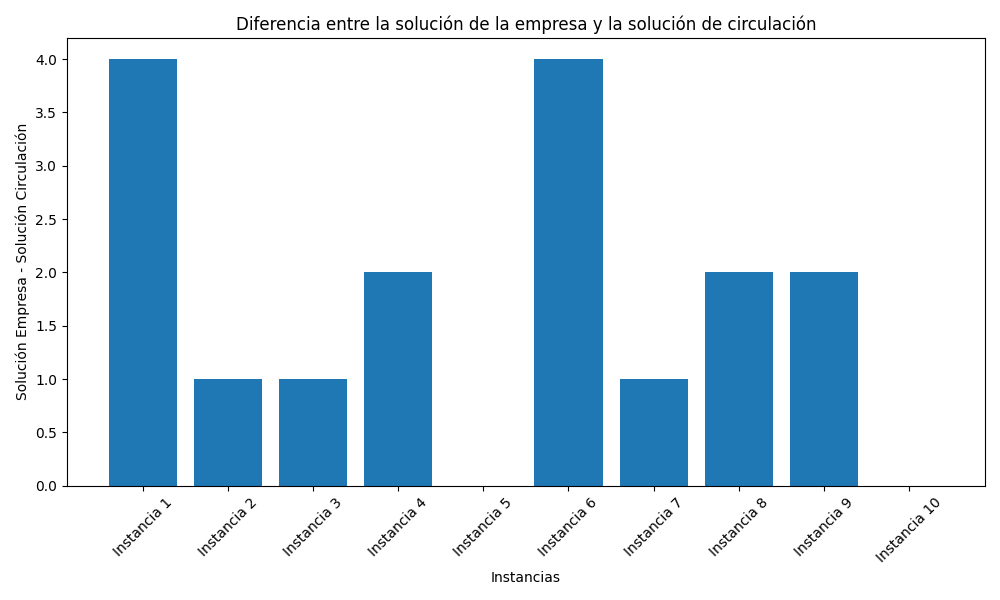
\includegraphics[width=0.6\textwidth]{exp1/plot_mediaAlta.png}
    \caption{Diferencias entre la solucion de la empresa y la solucion de circulacion (media alta)}
    \label{fig:ejemplo}
\end{figure}

Se repitió el proceso para demandas normales con media 500 (instancias y resultados en \texttt{experimentacion\_e\_informe} $/$ \texttt{exp1} $/$ \texttt{media\_baja}). Los resultados obtenidos son similares a los de la media alta:

\begin{figure}[H]
    \centering
    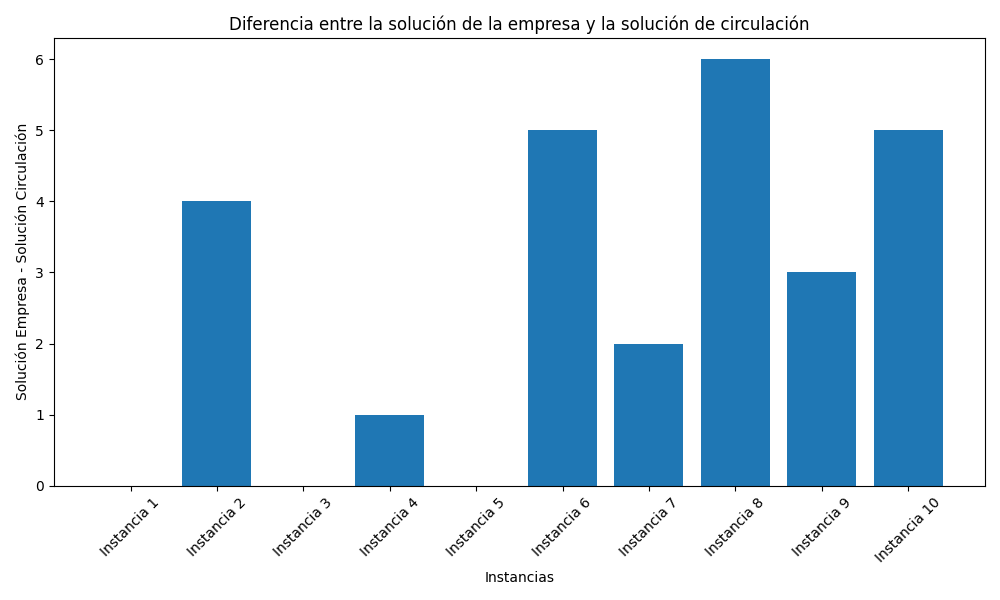
\includegraphics[width=0.6\textwidth]{exp1/plot_mediaBaja.png}
    \caption{Diferencias entre la solucion de la empresa y la solucion de circulacion (media baja)}
    \label{fig:ejemplo}
\end{figure}

Como se ve las diferencias son en ambos casos siempre mayores o iguales a 0. Por ello, concluimos que, como se esperaba, el modelo propuesto genera, tanto para demandas altas como bajas, mejores soluciones al problema. Como observación adicional, no pareciera que el nivel de la demanda (alta o baja) modifique esa mejoría en las respuestas. Para ambos niveles, la mejoría (diferencia) estuvo entre 0 y 6 unidades rodantes.

\subsection*{Experimento 2: Análisis de la Cantidad de Unidades Nuevas vs. Demanda}

Se busca evaluar cómo varía la cantidad de unidades nuevas necesarias para cubrir la demanda cuando se incrementa la demanda de los servicios. Nuestra hipótesis es que aprovechado el traspaso de unidades entre eventos, al aumentar linealmente la demanda media de las instancias, la cantidad de unidades nuevas necesarias aumentará de forma menor que lineal.

Para esto, se generaron diez instancias para cada tipo de demanda media: baja (500), media-baja (1000), media-alta (1500) y alta (2000) (siempre cuidando que los valores estén entre 0 y 2500 que es el máximo por la capacidad de la red). Luego se corrió el modelo de circulación para cada instancia y se promedió la cantidad de unidaes necesarias por tipo de demanda.Las instancias y los archivos con la implementación del experimento están en \texttt{experimentacion\_e\_informe} $/$ \texttt{exp2}.  Los resultados se presentan a continuación:

\begin{figure}[H]
   \centering
    \begin{minipage}{0.45\textwidth}
        \centering
        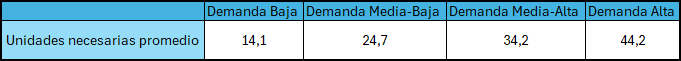
\includegraphics[width=\textwidth]{exp2/unidades_promedio.png}
        \caption{Unidades necesarias promedio por tipo de demanda}
        \label{fig:grafico1}
    \end{minipage}
    \hfill
    \begin{minipage}{0.45\textwidth}
        \centering
        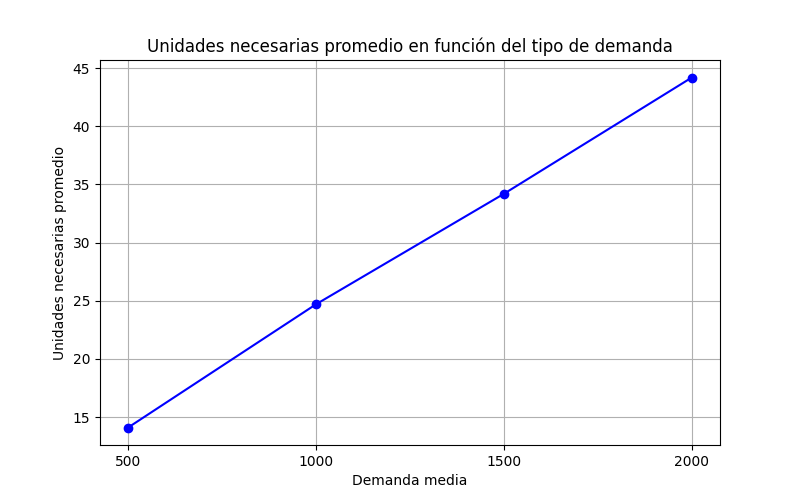
\includegraphics[width=\textwidth]{exp2/plot_unidades_promedio.png}
        \caption{Curva de unidades necesarias promedio en función de la demanda media}
        \label{fig:grafico2}
    \end{minipage}
    \label{fig:dos_graficos}
\end{figure}

Como se puede apreciar, medida que la demanda media aumenta linealmente (saltos de 500 pasajeros), la cantidad de unidades necesarias promedio para cubrir la demanda también lo hace. Así, nuestra hipótesis no puede ser comprobada.

\subsection*{Experimento 3: Impacto de las Cotas Máximas en la Utilización del Material Rodante}

La idea es analizar cómo afectan las restricciones de las cotas máximas en los servicios a la solución óptima. Nuestra hipótesis es que disminuir la cota máxima de los servicios forzará un aumento en la cantidad de unidades nuevas, ya que se limitará la reutilización del material rodante.

Para este experimento generamos 10 csv con demanda media 500 y desvío estándar 200, y los convertimos a instancias con distintas cotas máximas. Las cotas utilizadas fueron: 25, 20, 15, 10. Luego se corrió el modelo de circulación sobre todas las instancias y se promedió la cantidad de unidades necesarias para cada una de las cotas. El resultado se muestra en la siguiente tabla:

\begin{figure}[H]
    \centering
    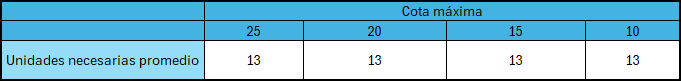
\includegraphics[width=0.6\textwidth]{exp3/unidades_promedio.png}
    \caption{Unidades necesarias promedio para distintas cotas máximas}
    \label{fig:ejemplo}
\end{figure}

Al contrario de lo esperado, no varió la cantidad de unidades necesitadas. Luego de mirar con detenimiento lo que pasaba en distintas instancias, vimos que si bien ocurría que se modificaba la cantidad de flujo circulante entre los eventos del día, este cambio se compensaba con los viajes añadidos de final del dia entre estaciones, que tienen capacidad ilimitada.

\subsection*{Experimento 4: Evaluación del Costo del Traspaso Nocturno}

Queremos estudiar el impacto del costo asociado a los traspasos nocturnos en la cantidad de unidades utilizadas. Que los costos de los arcos de trasnoche no sea el mismo para ambas estaciones, representaría que hay una estación en la que es más costoso dejar los trenes para que pasen la noche. Nuestra hipótesis es que para demandas bajas en relación a la capacidad máxima de la red, se podrá ajustar el flujo con los arcos del día para maximizar el uso de los arcos de trasnoche baratos y mantener mínimo el costo total, mientras que para demandas altas será inevitable tener que usar los arcos de trasnoche más caros.

Para este experimento usamos los mismos csv del experimento 1 para la demanda baja y generamos diez nuevos con demanda normal con media 1800 y desvío estándar 200 para la demanda alta. Al convertir los csv a instancias, lo hicimos una vez con costos de los arcos de trasnoche iguales  y una vez con un costo mayor al otro. Así, se obtienen dos configuraciones de costos, $costos_1 = (1, 1)$ y $costos_2 = (1, 2)$ para cada cronograma.  

Luego, se resolvió el problema para todas las instancias, obteniendo para cada cronograma una cantidad de unidades necesarias con la configuración $costos_1$ (la llamaremos $\#c_1$) y una cantidad de unidades necesarias con la configuración $costos_1$ (la llamaremos $\#c_2$).

Finalmente, para cada cronograma, se calcula la proporción de aumento en las unidades necesarias como $\frac{\#c_1}{\#c_2}$. La implementación del experimento, las instancias y los resultados se encuentran en \texttt{experimentacion\_e\_informe} $/$ \texttt{exp3}. Adeás, se muestran los resultados a continuación en forma de boxplot:

\begin{figure}[H]
    \centering
    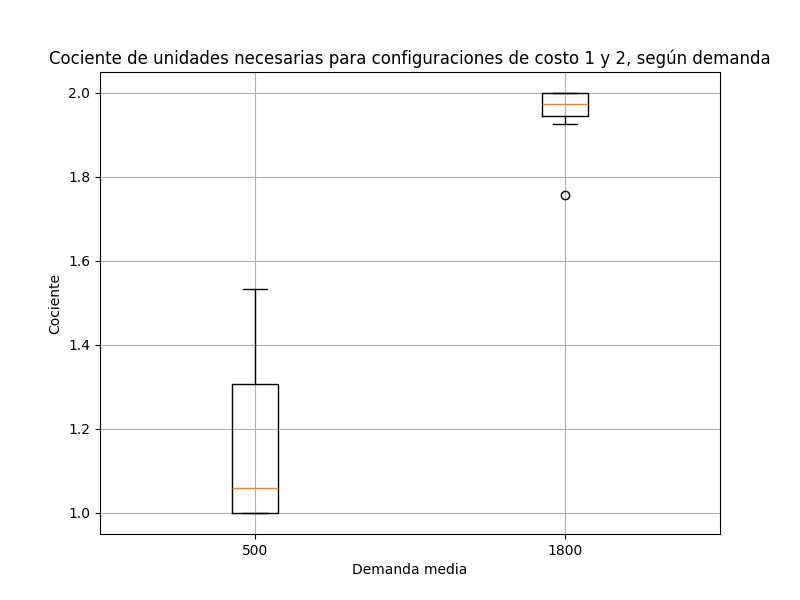
\includegraphics[width=0.6\textwidth]{exp4/cocientes.png}
    \caption{Cociente $\frac{\#c_1}{\#c_2}$, según la demanda}
    \label{fig:ejemplo}
\end{figure}

Como se esperaba, parece haber evidencia de que el aumento proporcional es mayor para demandas altas que para demandas bajas. 

\subsection*{Experimento 5: Escalabilidad del modelo}

Se desea evaluar cómo varía el tiempo de ejecución del algoritmo al aumentar el tamaño del problema (número de servicios y estaciones). Se espera que el tiempo de ejecución aumente de forma polinómica con el tamaño del problema debido a la complejidad del algoritmo de flujo de costo mínimo.

Para esto se consideraron distintos tamños de entrada para el problema: 500, 1000, 2000, 5000, 10000 y 20000 eventos de salida para cada estación. Se eligió usar tiempos para los eventos aleatorios y demandas con distribución normal de media 1000 y desvío estandar 200.

Luego, para cada tamaño de entrada posible se tomó 5 veces el tiempo de ejecución de \texttt{modelo\_circulacion()} y se tomó el promedio de dichos tiempos. Los resultados se presentan a continuación:

\begin{figure}[H]
    \centering
    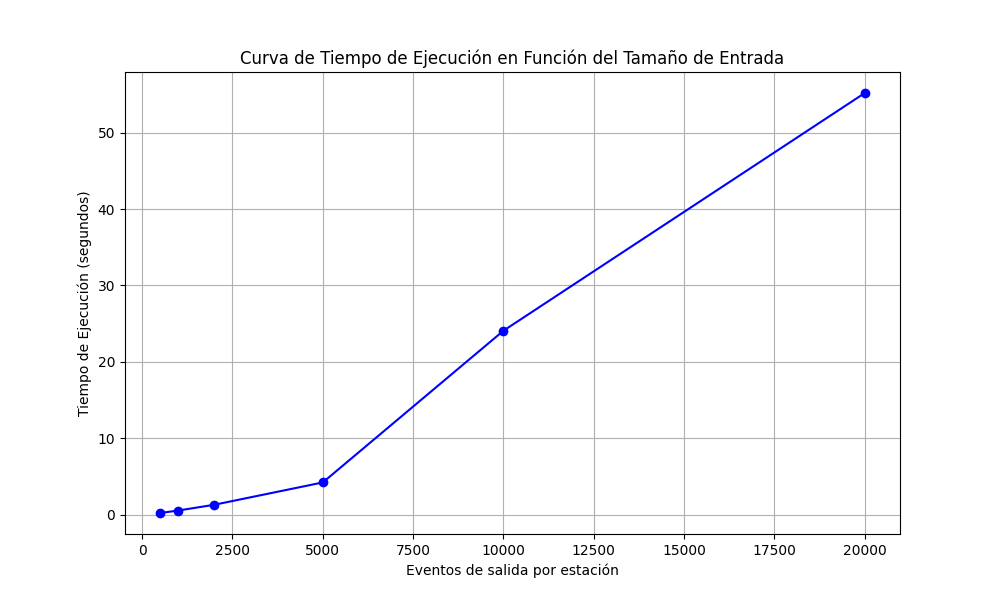
\includegraphics[width=0.6\textwidth]{exp5/tiempos.png}
    \caption{Tiempo de ejecución del modelo según el tamaño de entrada}
    \label{fig:ejemplo}
\end{figure}

Si bien resulta evidente que el tiempo de ejecución no es lineal en el tamaño de la entrada, tampoco resulta evidente ver a qué clase de polinomio se aproxima. La profundización en el estudio de la complejidad temporal del algoritmo puede ser tema para futuros experimentos y trabajos.

\section*{Sección 4: Escenario adicional}

En el escenario adicional planteado por la cátedra, se considera la operación conjunta de diferentes ramales dentro de la línea Mitre. Actualmente, cada ramal opera de manera independiente, utilizando su propio material rodante sin compartir recursos entre los ramales. La empresa ferroviaria busca evaluar si sería más conveniente unificar la operación de los ramales, permitiendo el uso compartido del material rodante a lo largo de toda la línea Mitre. Este cambio implicaría que el material rodante pueda quedar estacionado durante la noche en cualquiera de las cuatro estaciones principales (Retiro, Mitre, Victoria, y Cardales), lo que podría mejorar la reutilización de los recursos y reducir el número total de unidades necesarias. El análisis de este escenario permite estudiar el impacto de la decisión en términos de costos, eficiencia operativa, y capacidad para satisfacer la demanda. 

El escenario se muestra mejor en el siguiente esquema:

\begin{figure}[H]
    \centering
    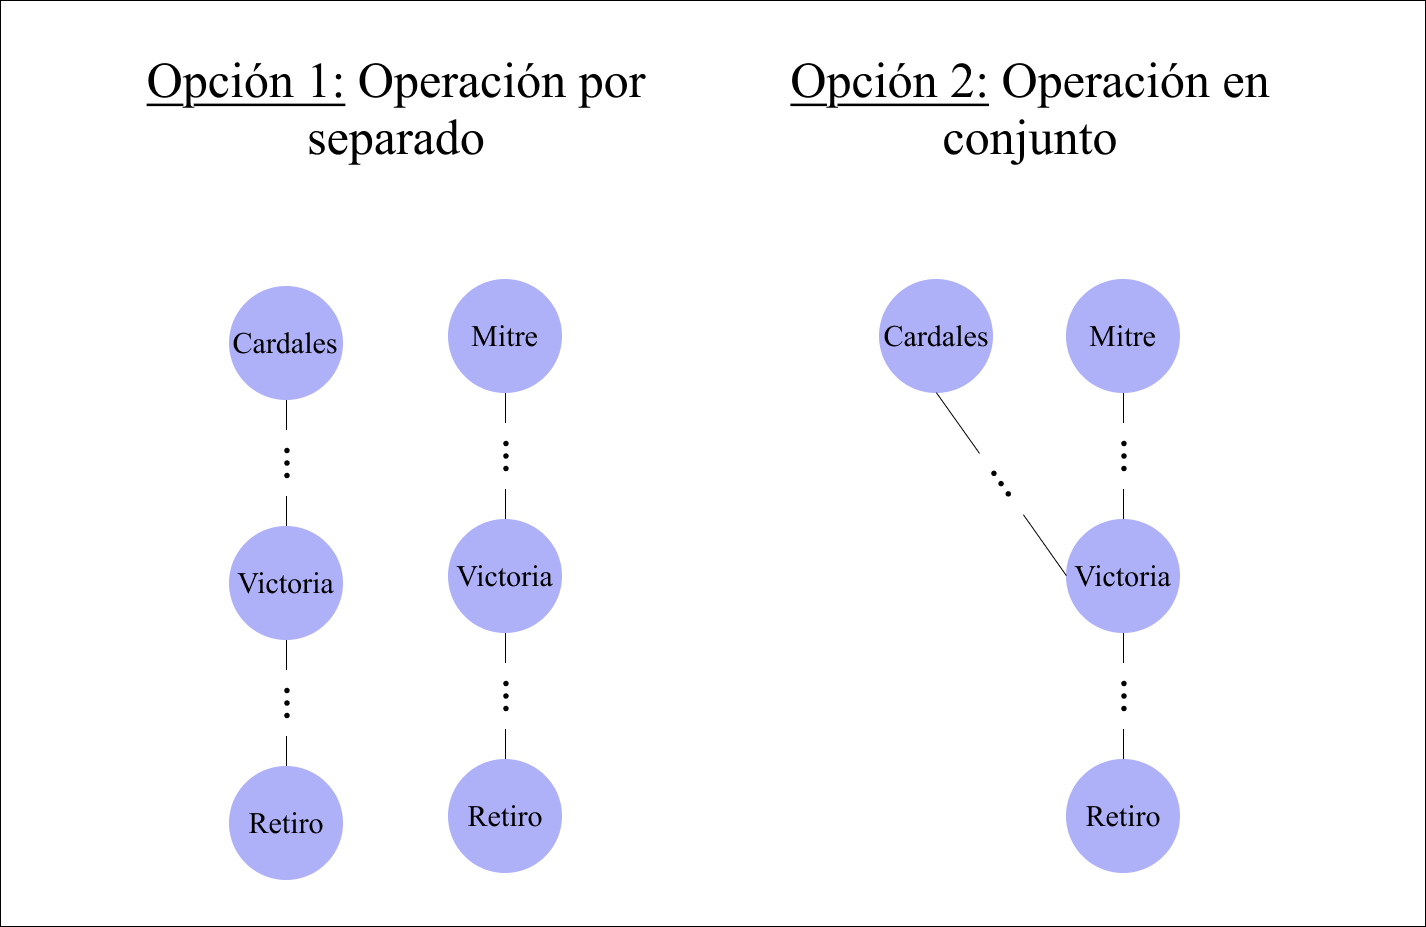
\includegraphics[width=0.6\textwidth]{esquema_escenario_adic.png}
    \caption{Opciones para la gestión de las unidades de la línea Retiro-Mitre y sus ramales}
    \label{fig:ejemplo}
\end{figure}

Nosotros proponemos que operar las líneas juntas solo puede traer beneficios a la empresa. Al poder decidir si operar los ramales como una sola línea y compartir las unidades entre ramales o no, a lo sumo solo se puede reducir la cantidad de unidades rodantes necesarias en la línea.

A coninuación se muestra un cronograma de ejemplo donde se ve el beneficio de operar los ramales como una única linea con posibilidad de que el material rodante pase la noche en cualquiera de las estaciones.

\begin{figure}[H]
    \centering
    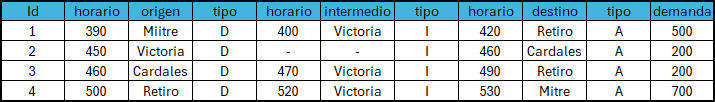
\includegraphics[width=0.6\textwidth]{escenario_adic_ejemplo.png}
    \caption{Cronograma de ejemplo}
    \label{fig:ejemplo}
\end{figure}

En el cronograma, a diferencia de antes, se indica un nuevo evento de tipo I (intermedio) para los servicios que pasan por la estación Victoria durante su recorrido. Si el servicio parte desde Victoria, no hay evento de tipo I. Para las soluciones, se asume que la capacidad de todos los arcos de tren es de 25 y que la capacidad de los vagones es de 100 unidades.

Si se operasen los dos ramales como líneas independientes, las soluciones (como flujos) serían las siguientes:

\begin{figure}[H]
   \centering
    \begin{minipage}{0.45\textwidth}
        \centering
        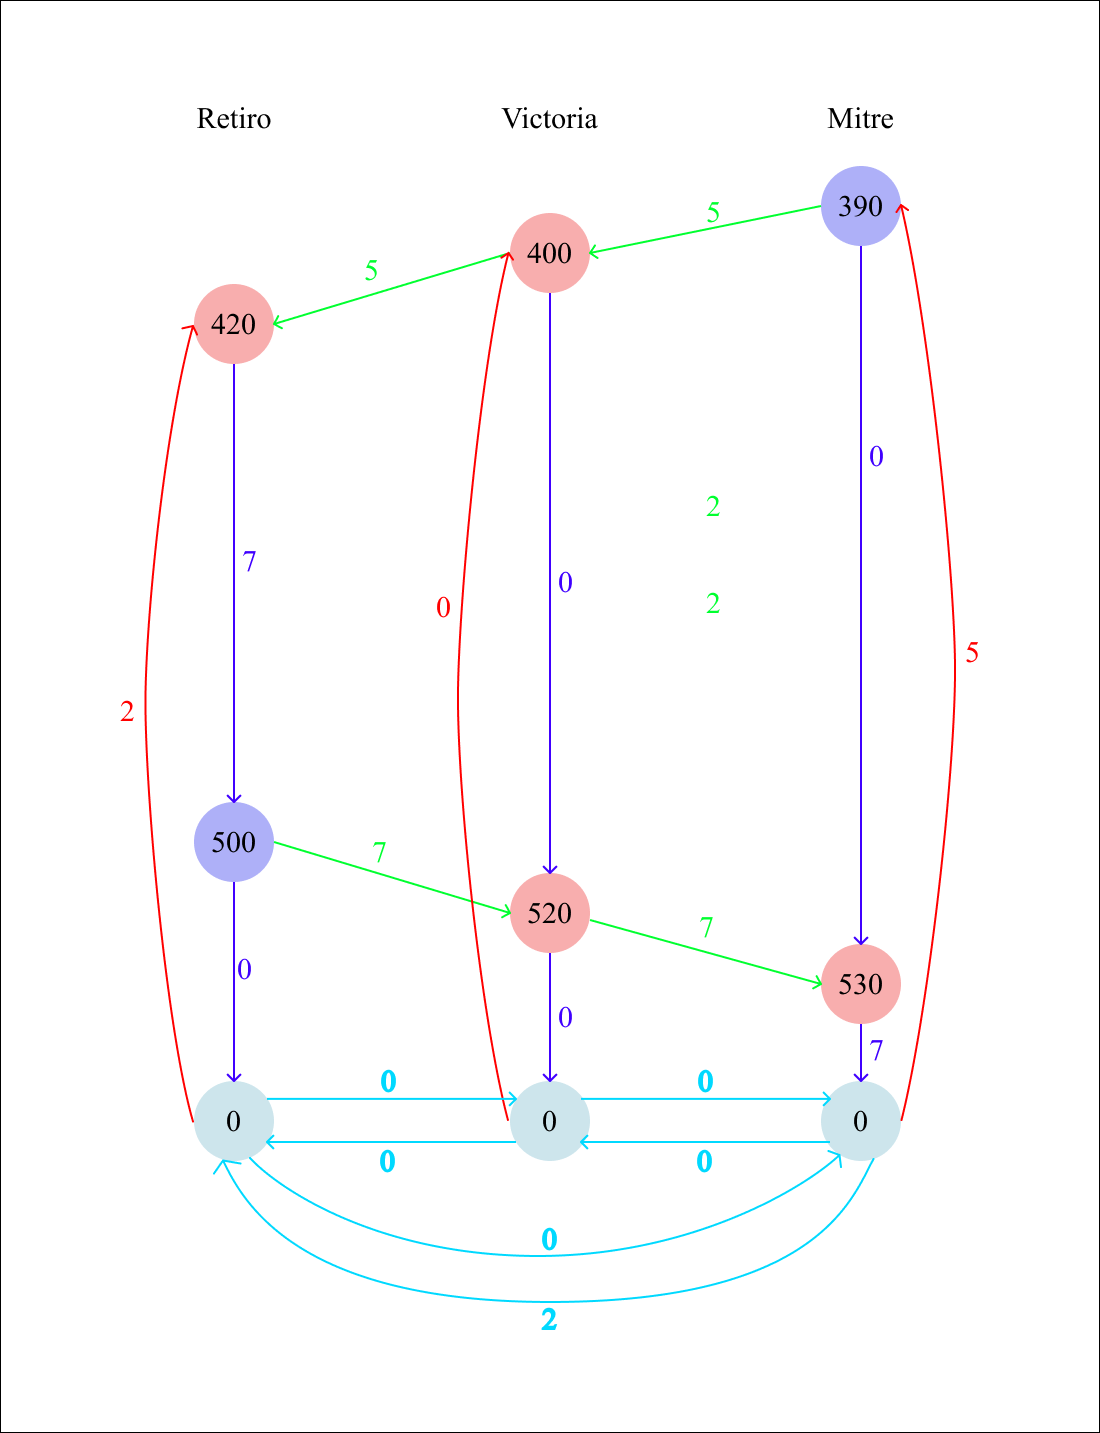
\includegraphics[width=\textwidth]{Retiro-Mitre.png}
        \caption{Ramal Retiro-Mitre}
        \label{fig:grafico1}
    \end{minipage}
    \hfill
    \begin{minipage}{0.45\textwidth}
        \centering
        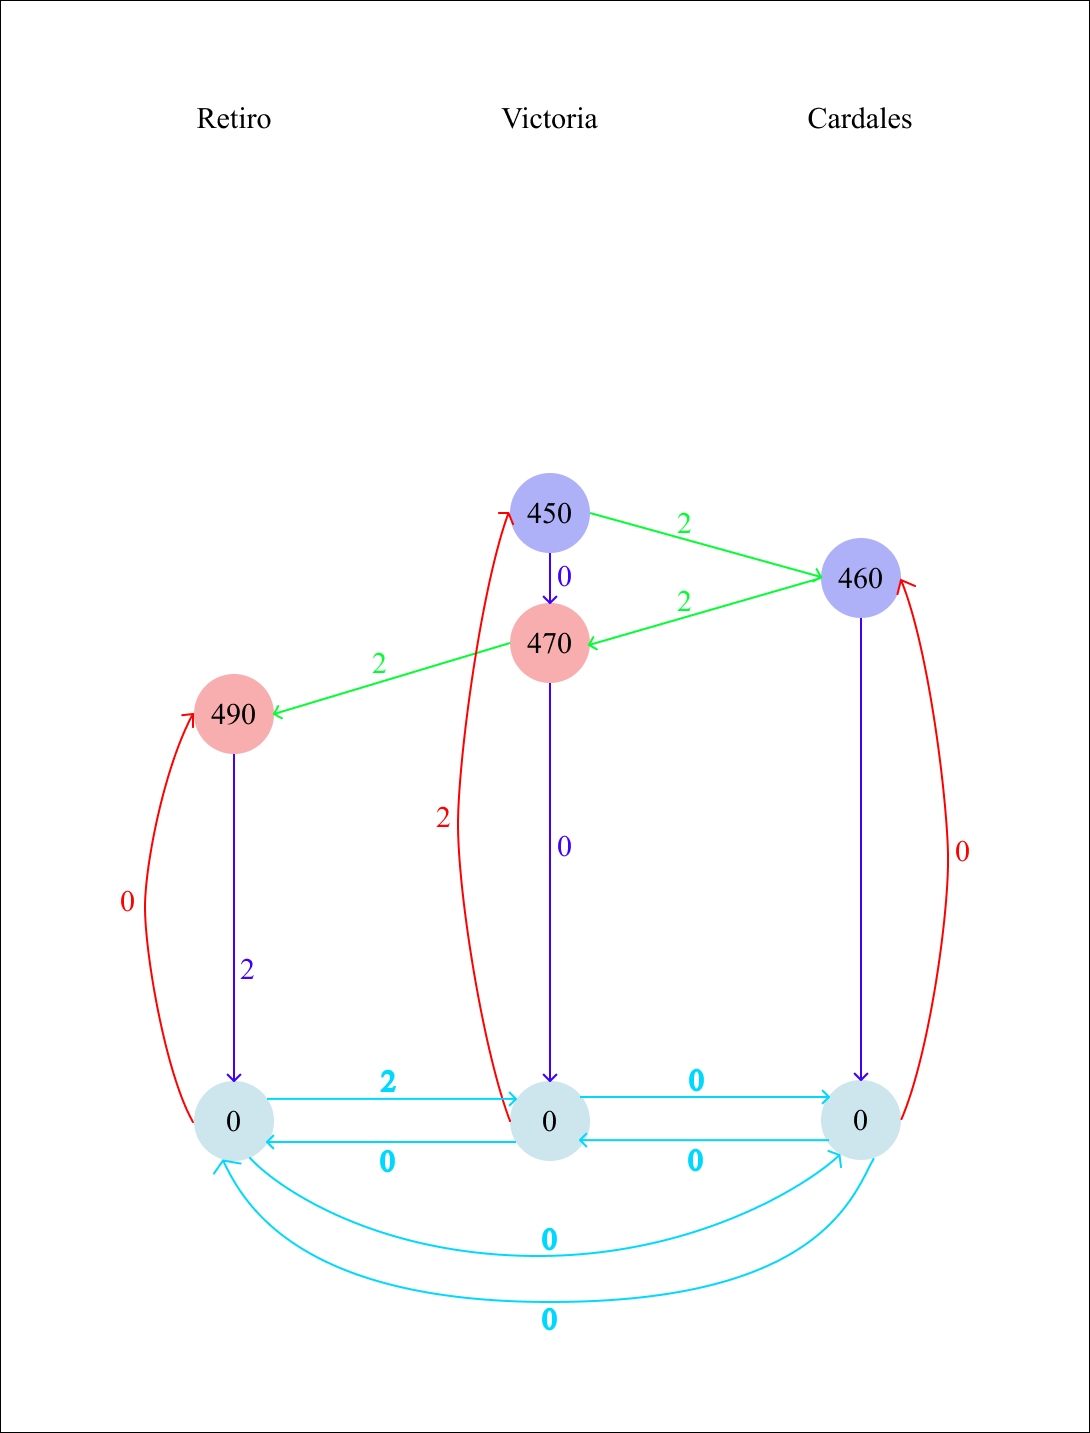
\includegraphics[width=\textwidth]{Retiro-Cardales.png}
        \caption{Ramal Retiro-Cardales}
        \label{fig:grafico2}
    \end{minipage}
    \label{fig:dos_graficos}
\end{figure}

Como se puede ver, en total se necesitarían 9 unidades rodantes para satisfacer la demanda de ambos ramales. Sin embargo, si se operasen los dos ramales como una sola línea con la posibilidad de compartir unidades entre eventos, la solución sería la siguiente:

\begin{figure}[H]
    \centering
    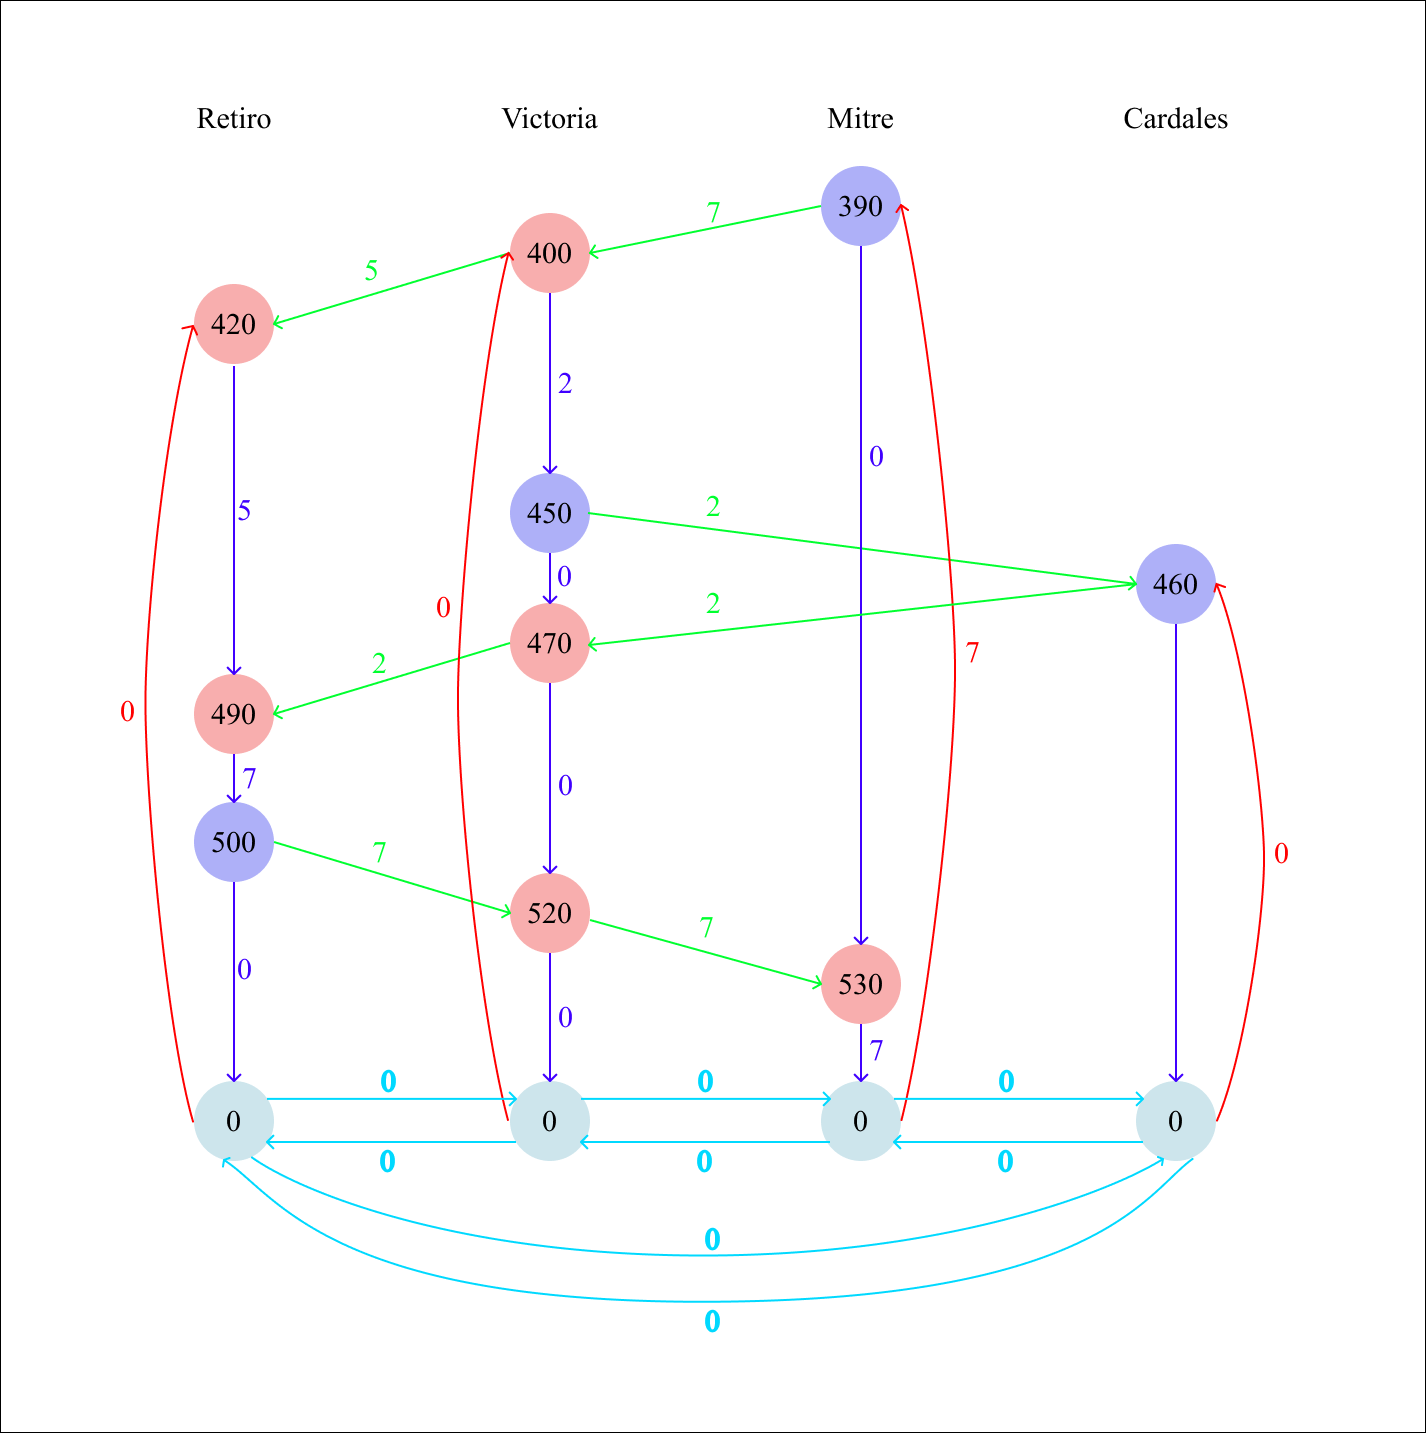
\includegraphics[width=0.55\textwidth]{ramales_juntos.png}
    \caption{Ramales como línea única}
    \label{fig:ejemplo}
\end{figure}

En esta solución se puede ver que se puede satisfacer la demanda de toda la línea con solo 7 unidades rodantes. Así, al administrar ambos ramales como uno solo, se logró utilizar menos material rodante.

\section*{Sección 5: Conclusiones}
En este trabajo, se desarrolló un modelo para la planificación eficiente del material rodante algoritmos de flujo de costo mínimo aplicados a un grafo espacio-temporal. A lo largo de los experimentos realizados, se pudo validar la efectividad del modelo propuesto en comparación con el método tradicional utilizado por la empresa, abordando distintos escenarios de demanda y restricciones operativas

También se encontró que aumentar el costo asociado a los traspasos nocturnos incentiva una mayor reutilización del material rodante durante el día. Este resultado indica que es posible reducir los costos operativos diarios ajustando adecuadamente las políticas de traspaso.

En el análisis del escenario adicional, al considerar la unificación de los ramales y el uso compartido del material rodante a lo largo de toda la línea Mitre, se observó una disminución significativa en la cantidad total de unidades necesarias. La implementación de un sistema compartido permitiría menores costos operativos y una mayor flexibilidad para satisfacer la demanda en horarios pico, lo que sugiere una ventaja clara respecto a la operación independiente de cada ramal.

A pesar de los resultados positivos, el estudio presenta algunas limitaciones. La simplificación del modelo, al asumir una capacidad infinita en las cabeceras y utilizar demandas generadas aleatoriamente, podría no reflejar completamente la complejidad de un cronograma real. Además, la complejidad temporal observada en el experimento de escalabilidad sugiere la necesidad de optimizar la implementación del algoritmo para manejar instancias más grandes con mayor eficiencia.

En futuros trabajos, sería interesante explorar la inclusión de eventos intermedios adicionales y considerar variaciones en la capacidad del material rodante para reflejar mejor las condiciones reales. También se podrían analizar métodos alternativos para reducir la complejidad temporal del algoritmo, lo que permitiría una mejor aplicación directa en contextos operativos reales.

\printbibliography

\end{document}